
\documentclass[12pt]{extarticle}
%%%%%%%%%%%%%%%%%%%%%%%%%%%%%%%%%%%%%%%%
% Environment settings
%%%%%%%%%%%%%%%%%%%%%%%%%%%%%%%%%%%%%%%%
\usepackage[utf8]{inputenc}
\usepackage{tikz}
\usepackage{CJKutf8}
\usepackage{amsmath}
\usepackage[shortlabels]{enumitem}
\usetikzlibrary{shapes.geometric, arrows}
\usetikzlibrary{positioning}

%%%%%%%%%%%%%%%%%%%%%%%%%%%%%%%%%%%%%%%%
% Tikz grpaher settings
%%%%%%%%%%%%%%%%%%%%%%%%%%%%%%%%%%%%%%%%

\tikzstyle{arrow} = [thick, ->, >=stealth]
\tikzstyle{player} = [circle, minimum width=1.5cm, text centered, draw=black]
\tikzstyle{bidder} = [circle, minimum width=1cm, text centered, draw=black]
\tikzstyle{state} = [rectangle, minimum height=1cm, text centered, draw=black]
\tikzstyle{chain} = [trapezium, trapezium left angle=70, trapezium right angle=110, minimum height=1cm, text centered, draw=black]

%%%%%%%%%%%%%%%%%%%%%%%%%%%%%%%%%%%%%%%%
% Title page
%%%%%%%%%%%%%%%%%%%%%%%%%%%%%%%%%%%%%%%%


\begin{document}
\begin{CJK*}{UTF8}{bkai}
\title{NMLab Final Project Proposal \\ DApp: BidChain}
\author{黃品文, 姚慶旺, 張力文}
\date{May 2020}
    \maketitle

    \section*{Introduction}
        BidChain is a bidding system based on Ethereum smart contracts. Using a decentralised structure to ensure the fair of competition. 
        Both sellers and buyers' rights are protected under our smart contract.

    \subsection*{Solidity API(external functions used by web3)}
        \begin{enumerate}[(a)]
            \item setPrice(address account, uint price, uint goodsId)
            \item bidding(address account, uint price, uint goodsId)  returns (bool, uint)
            \item getPrice(uint goodsId) external view returns(uint)
            \item getGoods() external view returns (uint[])
            \item winner(uint goodsId) external view returns(address)
            \item getHistory() external view returns(address[], uint[])
            \item queryIfGet(bool ) external returns()
        \end{enumerate}

    \section*{Process Diagram}
    	\begin{center}
        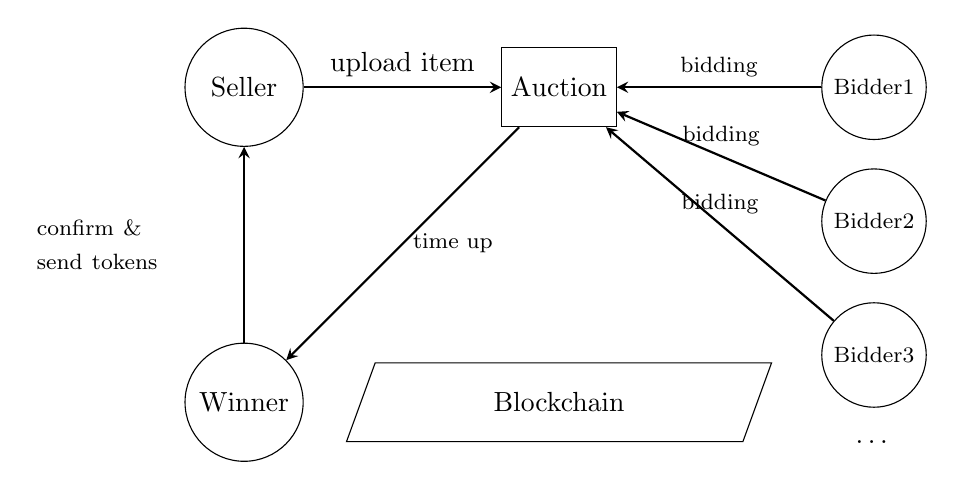
\begin{tikzpicture}[node distance=4cm]
          

            \node (SELLER) [player] {Seller};
            \node (AUCTION) [state, right of=SELLER] {Auction};
            \node (CHAIN) [chain, below of=AUCTION, text width=2cm] {Blockchain};
            \node (WINNER) [player, below of=SELLER] {Winner};
            \node (BIDDER1) [bidder, right of=AUCTION] {\footnotesize{Bidder1}};
            \node (BIDDER2) [bidder, right of=AUCTION, yshift=-1.7cm] {\footnotesize{Bidder2}};
            \node (BIDDER3) [bidder, right of=AUCTION, yshift=-3.4cm] {\footnotesize{Bidder3}};
            \node (DOTDOTDOT) [right of=AUCTION, yshift=-4.5cm] {\ldots};
        
            \draw [arrow] (SELLER) -- node [above] {upload item} (AUCTION);
            \draw [arrow] (BIDDER1) -- node [above] {\footnotesize{bidding}} (AUCTION);
            \draw [arrow] (BIDDER2) -- node [above] {\footnotesize{bidding}} (AUCTION);
            \draw [arrow] (BIDDER3) -- node [above] {\footnotesize{bidding}} (AUCTION);
            \draw [arrow] (AUCTION) -- node [right] {\footnotesize{time up}} (WINNER);
            \draw [arrow] (WINNER) -- node [left, text width=2.5cm] {\footnotesize{confirm \&\\ send tokens}} (SELLER);

        	
        \end{tikzpicture}
        \end{center}

\end{CJK*}
\end{document}

